\chapter{Testing, Validation, and Performance Analysis}\label{chap:Testing, Validation, and Performance Analysis}

This section deals with the evaluation of the solution described above, including hardware verification and performance analysis, and is performed using an experimental method.
Since the hardware architecture and implementation have already been described in the previous chapter, the main purpose of this section is to empirically demonstrate the validity of the proposed solution.
The demonstration concerns the solution's ability to achieve real-time stability, withstand system-induced delays, and remain unaffected by thermal or mechanical frictional shifts acting on the Double Crystal Monochromator (DCM).

The solution validation was performed in several ways through simulation benchmarks, system hardware telemetry, and beamline diagnostic measurements.

This section is divided into sections so that each of them contains a validation sextant part.
The first part is the experimental testbench and data acquisition, then the second part involves analyzing the synthetic structure used within the FPGA. This means investigating the amount of resources used and the timing closure.
Next, we analyze the pipeline used by the system to filter and demodulate the input signal before it is passed to the PID.
At the same time, we investigate the delay calibration to maintain synchrony between the dither and the reference signal.
As a final step, the robustness of the solution in the presence of disturbances will be demonstrated, as well as its convergence capacity and, for completeness, the functionality of the graphical interface in showing the first derivative will also be demonstrated.
\section{Experimental Setup and Methodology}

To make the experiment rigorous and deterministic, a simulation-based methodology was adopted. 
This ensures reproducibility of the experiments for validating the controller's stability and its demodulation performance in phase-sensitive situations.
Another advantage of using Software-in-the-Loop (SIL) is the elimination of a physical validation system, which in this case would be a synchrotron. 
The use of SIL in this case is interconnected with the solution itself given the complexity of the system. This means that the firmware has been partially modified for simulation purposes only; the controller itself functions exactly as it would in a real-world scenario.

\subsection{Closed-Loop Simulation Architecture (Mocked Plant)}
The simulation tries to model the physical scenario of a beamline and its problems such as thermal displacement and mechanical friction that slowly moves the monochromator thus shifting the position of the intensity peak:

\begin{itemize}
    \item \textbf{Position Output Generation:} The firmware inside the softcore that takes care of the intensity control only calculates how much the monochromator has to move to cancel the error.
    \item \textbf{Rocking Curve Intensity Modeling:} Instead of reading the beam intensity, the system utilizes the input. Instead of reading the intensity value passed by the TetrAMM, the value is overridden with a mathematical function representing the rocking curve of the beamline.
    This function dynamically calculates the expected photon beam intensity ($I$) corresponding to the specified crystal angle and time; time is useful for representing thermal or other types of displacement.
    \begin{equation}
        rock-curve-equation
    \end{equation}
    \item \textbf{State and Parameter Management:} 
    For the simulation to work, it is necessary to save the position of the monochromator inside the FPGA, since the current intensity will then be calculated using it in the next iteration.
    Time must also be saved since the rocking curve is also based on it, thanks to the time variable it is possible to shift the graph and consequently move the intensity peak over time.
    \item \textbf{Feedback Ingestion:} 
    Once the beam intensity has been simulated, the control system behaves as in the real case: it reads the intensity, then applies the pipeline to extract the derivative gradient from the signal, and then applies the PID to obtain the correction to send to the piezoelectric along with the dither signal.
    In the simulation, instead of sending the correction, it is added to the position saved within the firmware and then used to calculate the intensity using the rocking curve mathematical function.
\end{itemize}


\subsection{State Tracking and Controller Configuration}

Another advantage of simulation validation is the effectiveness in finding problems as there cannot be physical errors such as in the DCM double crystal monochromator.
Of course, in order to simulate the physical system it is necessary to save the position of the monochromator, since the purpose of the controller is to make correction movements on the position of the monochromator.

\subsection{Validation Objectives}
Running a simulation allows you to evaluate the proposed system with different metrics:
\begin{enumerate}
    \item How well the filters inside the pipeline can isolate the dither frequency without introducing an unstable phase shifts.
    \item Verify the accuracy of the system-induced delay calibration phase and test whether the control system can compensate for this delay.
    \item Once the monochromator has reached the position where the intensity peak is produced, measure the convergence time and the reliability versus jitter of the PID.
\end{enumerate}

\subsection{Transition to Real-World Operation}
While the simulated system was useful to empirically demonstrate the validity of the proposed solution, it still remains an intermediate validation method even if it includes the delay calibration phase.
During the implementation phase of the system in a real environment, it will be necessary to remove all the modified part inside the firmware so as not to compromise correct functioning.
The intensity will return to be provided by the TetrAMM and will represent the beam intensity read by the beam position monitor (BPM). 
The output will be the control signal produced by the PID plus the dither signal in volts and will be passed to the PreDAC, which will influence the piezoelectric connected to the second crystal of the double crystal monochromator (DCM).

\section{FPGA Resource Utilization and Timing Verification}

The main purpose of this thesis is to empirically demonstrate the validity of the thesis itself and therefore focuses on the peak intensity behavior of the control loop and its implementation on a softcore. 
Therefore, it deals with areas more related to firmware or software rather than low-level digital hardware optimization, but despite this it is still necessary to demonstrate the physical feasibility of the Qsys after being modified to fit the proposed situation.

Since the implemented changes involve simple Avalon ST connections or MM connections, or the design of a simple logic block for outputting values and parameters useful at the end of the project, once the solution is used on real systems, it will no longer be necessary to send the parameters used for simulation, as they will then be used for analysis.
So summarizing through the Quartus II FPGA development software, it confirms that:
\begin{itemize}
    \item \textbf{Logic Element (LE) Overhead:} The added logic was a small fraction of what was already inside Qsys, leaving ample capacity for the pre-existing ELS Instruments position control infrastructure.
    \item \textbf{Memory and Register Allocation:} It was used already present slot that weren't used already present inside the shared memory, so it cannot have impacted performance.
    \item \textbf{Timing Closure:} The synthesized design successfully met all clock domain constraints (operating reliably at the system clock frequency), ensuring that the asynchronous handshaking and interrupt generation for the Nios II softcore introduced no critical path setup or hold violations.
\end{itemize}

Having verified the integrity of the FPGA structure and the feasibility of the modified architecture, we can now focus on the main objective of validating the proposed solution.
Testing the performance of the four-stage pipeline.

\section{Lock-in and Peak-Tracking Performance Evaluation}

The main purpose of this section is to validate the solution proposed, that is testing and analyzing the signal-processing pipeline.
Precisely the system was evaluated on its ability to manipulate the raw signal at the input to extract the gradient of the intensity beam dictated by the dither signal, nevertheless its own ability to lock into the peak of intensity of the rocking curve.
It is worth remembering that the output of the PID controller is what drives the piezoelectric, thus if some of the noise or distortion inside the stages of the pipeline pass through, they can impact the accuracy of the control system.

\subsection{Spectral Isolation and Filtering Performance}

The intensity signal simulated by the function given the monochromator position and time, includes a variety of components, some such as the dither signal is desired, others such as broadband uniform noise and low-frequency baseline drift are not.
Since evaluating individual pipeline states is difficult given the difficulty of reading intermediate data within the FPGA, the pipeline was taken and decomposed into a more suitable environment for validation and analysis, such as Python.
Here it was possible to demonstrate the effectiveness of the cascaded IIR filtering stages:
\begin{itemize}
    \item \textbf{Band-Pass Pre-Filtering:} The 4th-order Bessel band pass filter centered at the frequency of the dither signal managed to remove all the noise present inside of the signal both at high and low frequencies, it even managed to remove the DC offset of the rocking curve. The objective of the pass band filter centered into the dither signal's frequency is to retrieve a clean sinusoidal modulation, which its amplitude should scale proportionally with the local slope of the rocking curve. And this is what happened, as can be seen in the Figure[~\ref{fig:band pass validation}].

    \begin{figure}[htbp]
        \centering
        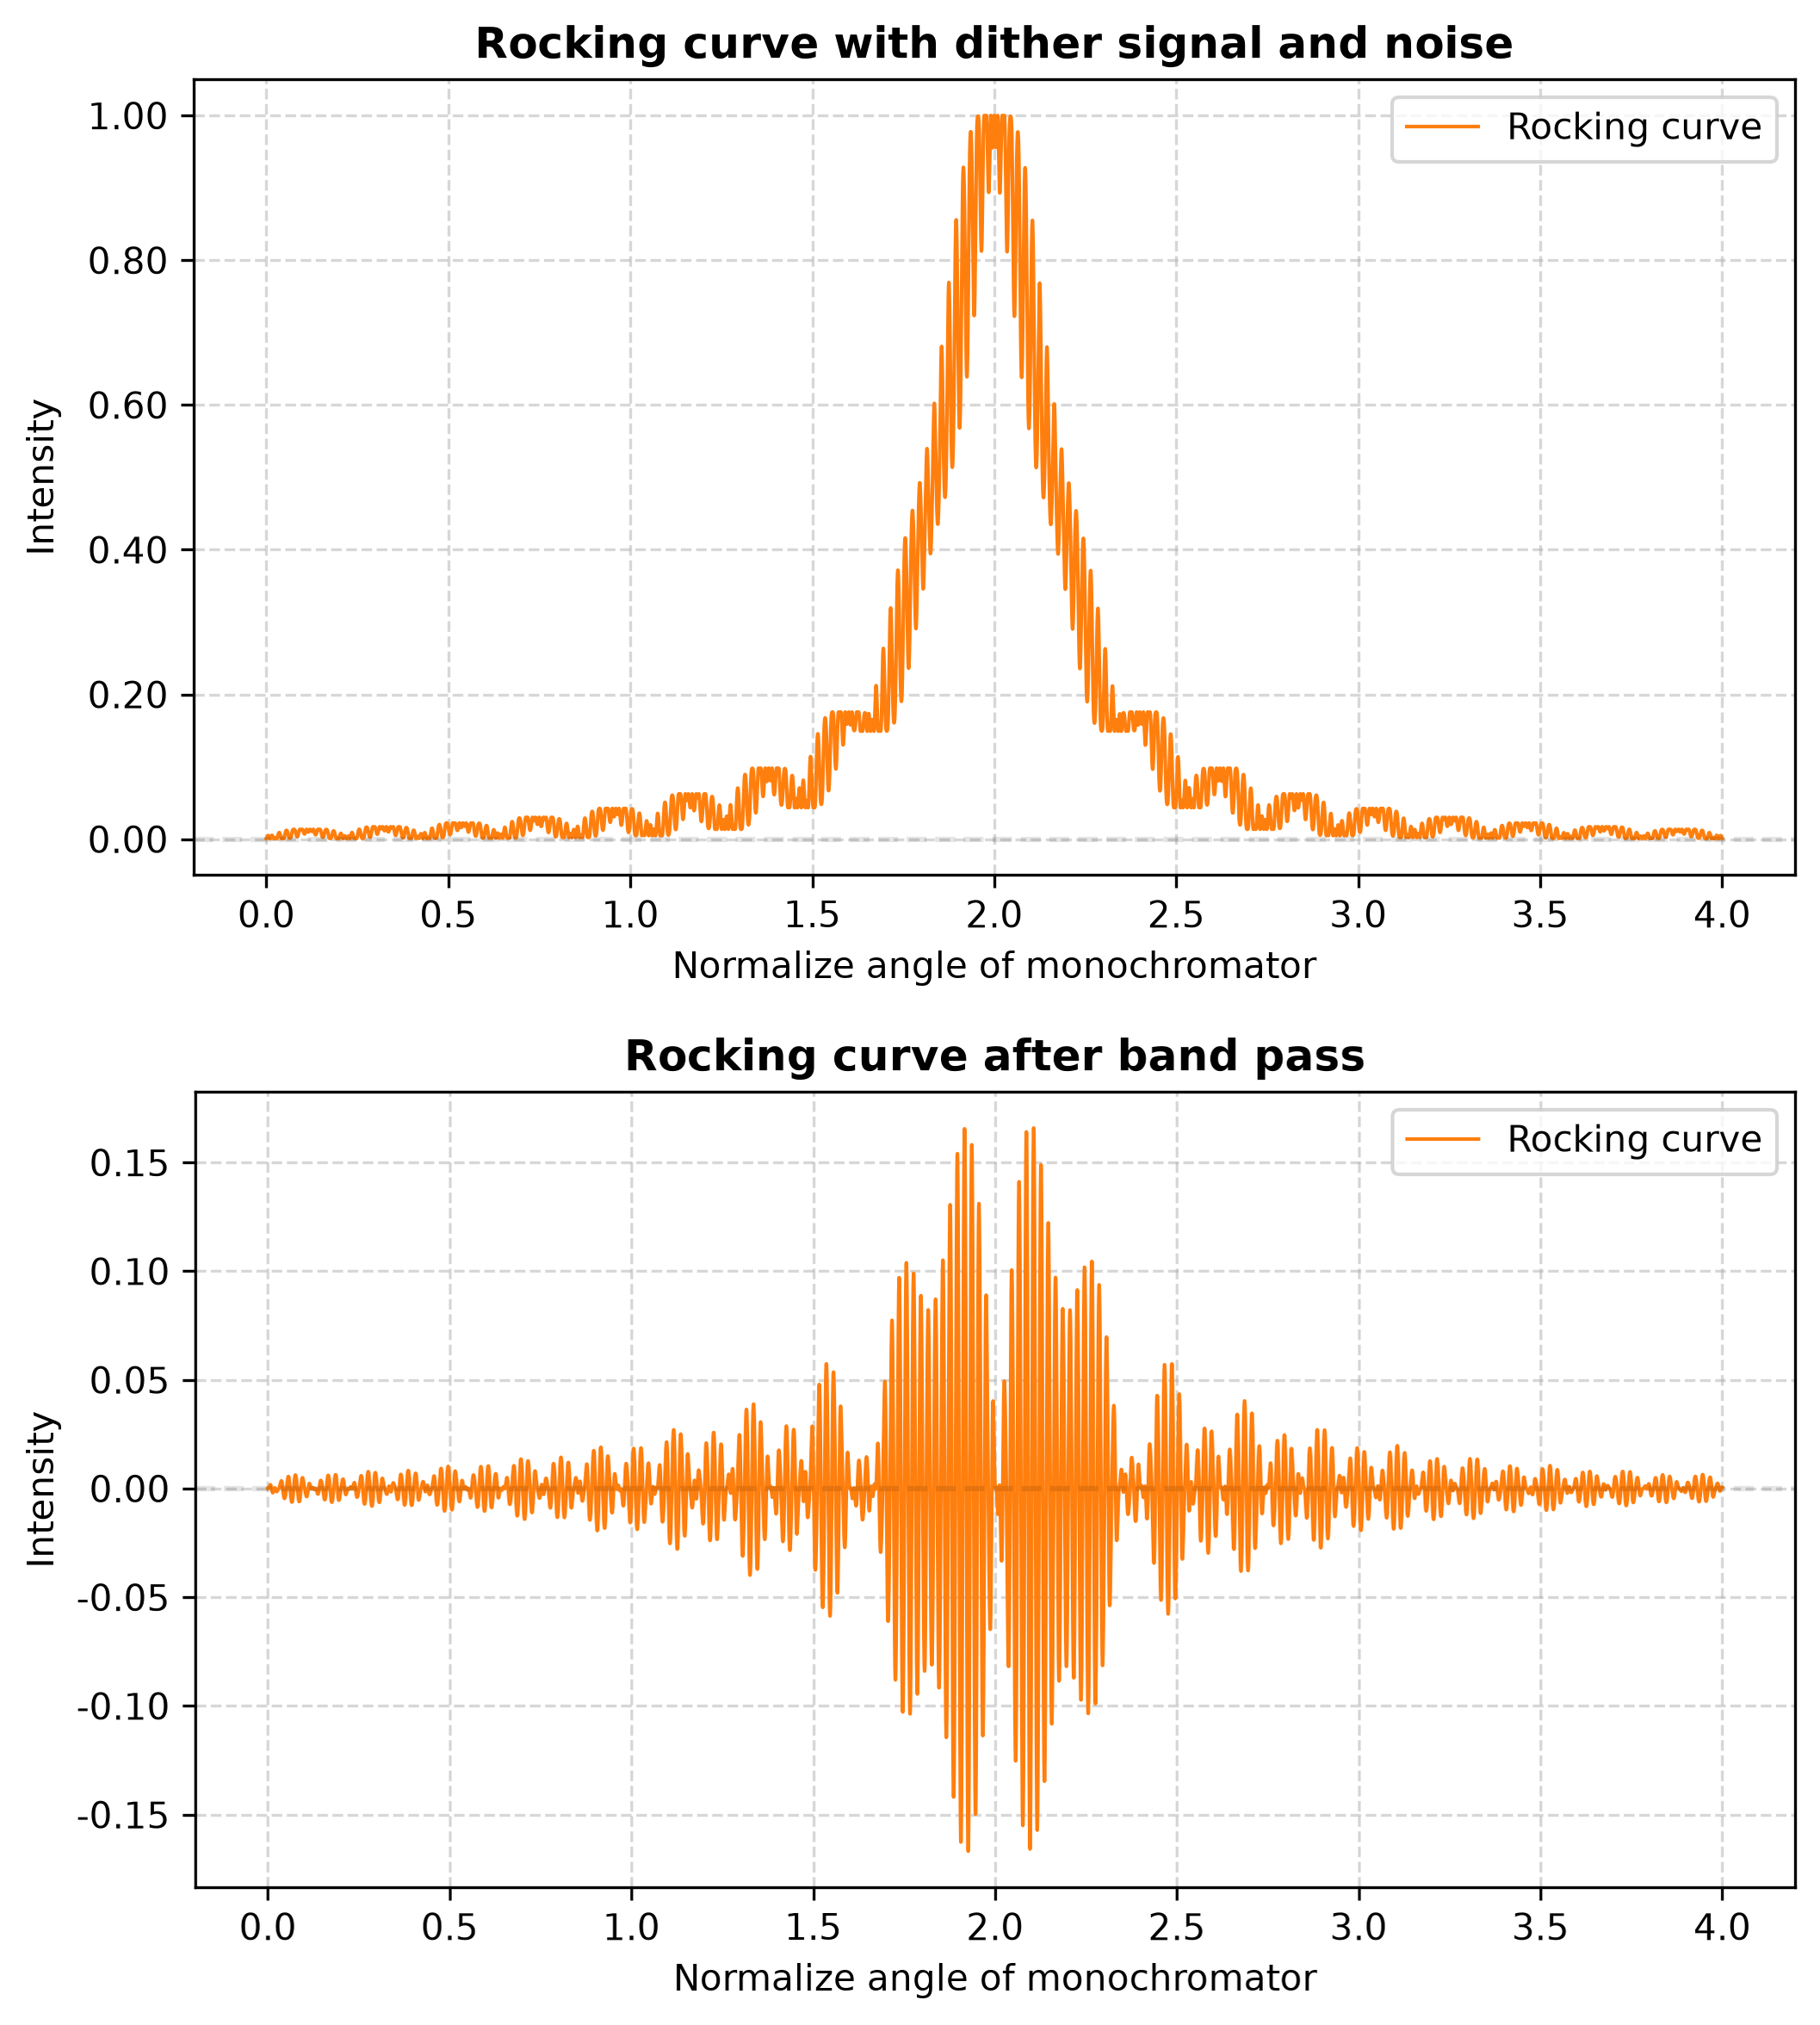
\includegraphics[width=0.85\textwidth]{img/cap 4/band_pass_validation.png}
        \caption{Comparison between before and after bandpass filtering. The input signal was injected with the dither signal and noise.}
        \label{fig:band pass validation}
    \end{figure}
    
    \item \textbf{Second-Harmonic Rejection:}  Mixing the intensity filtered by the pass band with the reference signal, which split the information at frequency $f_d$ into a DC offset and a $2f_d$ component. The mixed signal is then passed through a low pass filter for isolate the DC component which ca be identify in the gradient of the signal useful for the closed-loop integration.
\end{itemize}

\subsection{Gradient Extraction Accuracy ($dI/dt$ Linearity)}
To be analytically certain that the demodulated signal carries the information of the first derivative of intensity, a check was performed with an analytically calculated first derivative on the entire rocking curve, Figure[~\ref{fig:gradient validation}]. 

\begin{figure}[htbp]
    \centering
    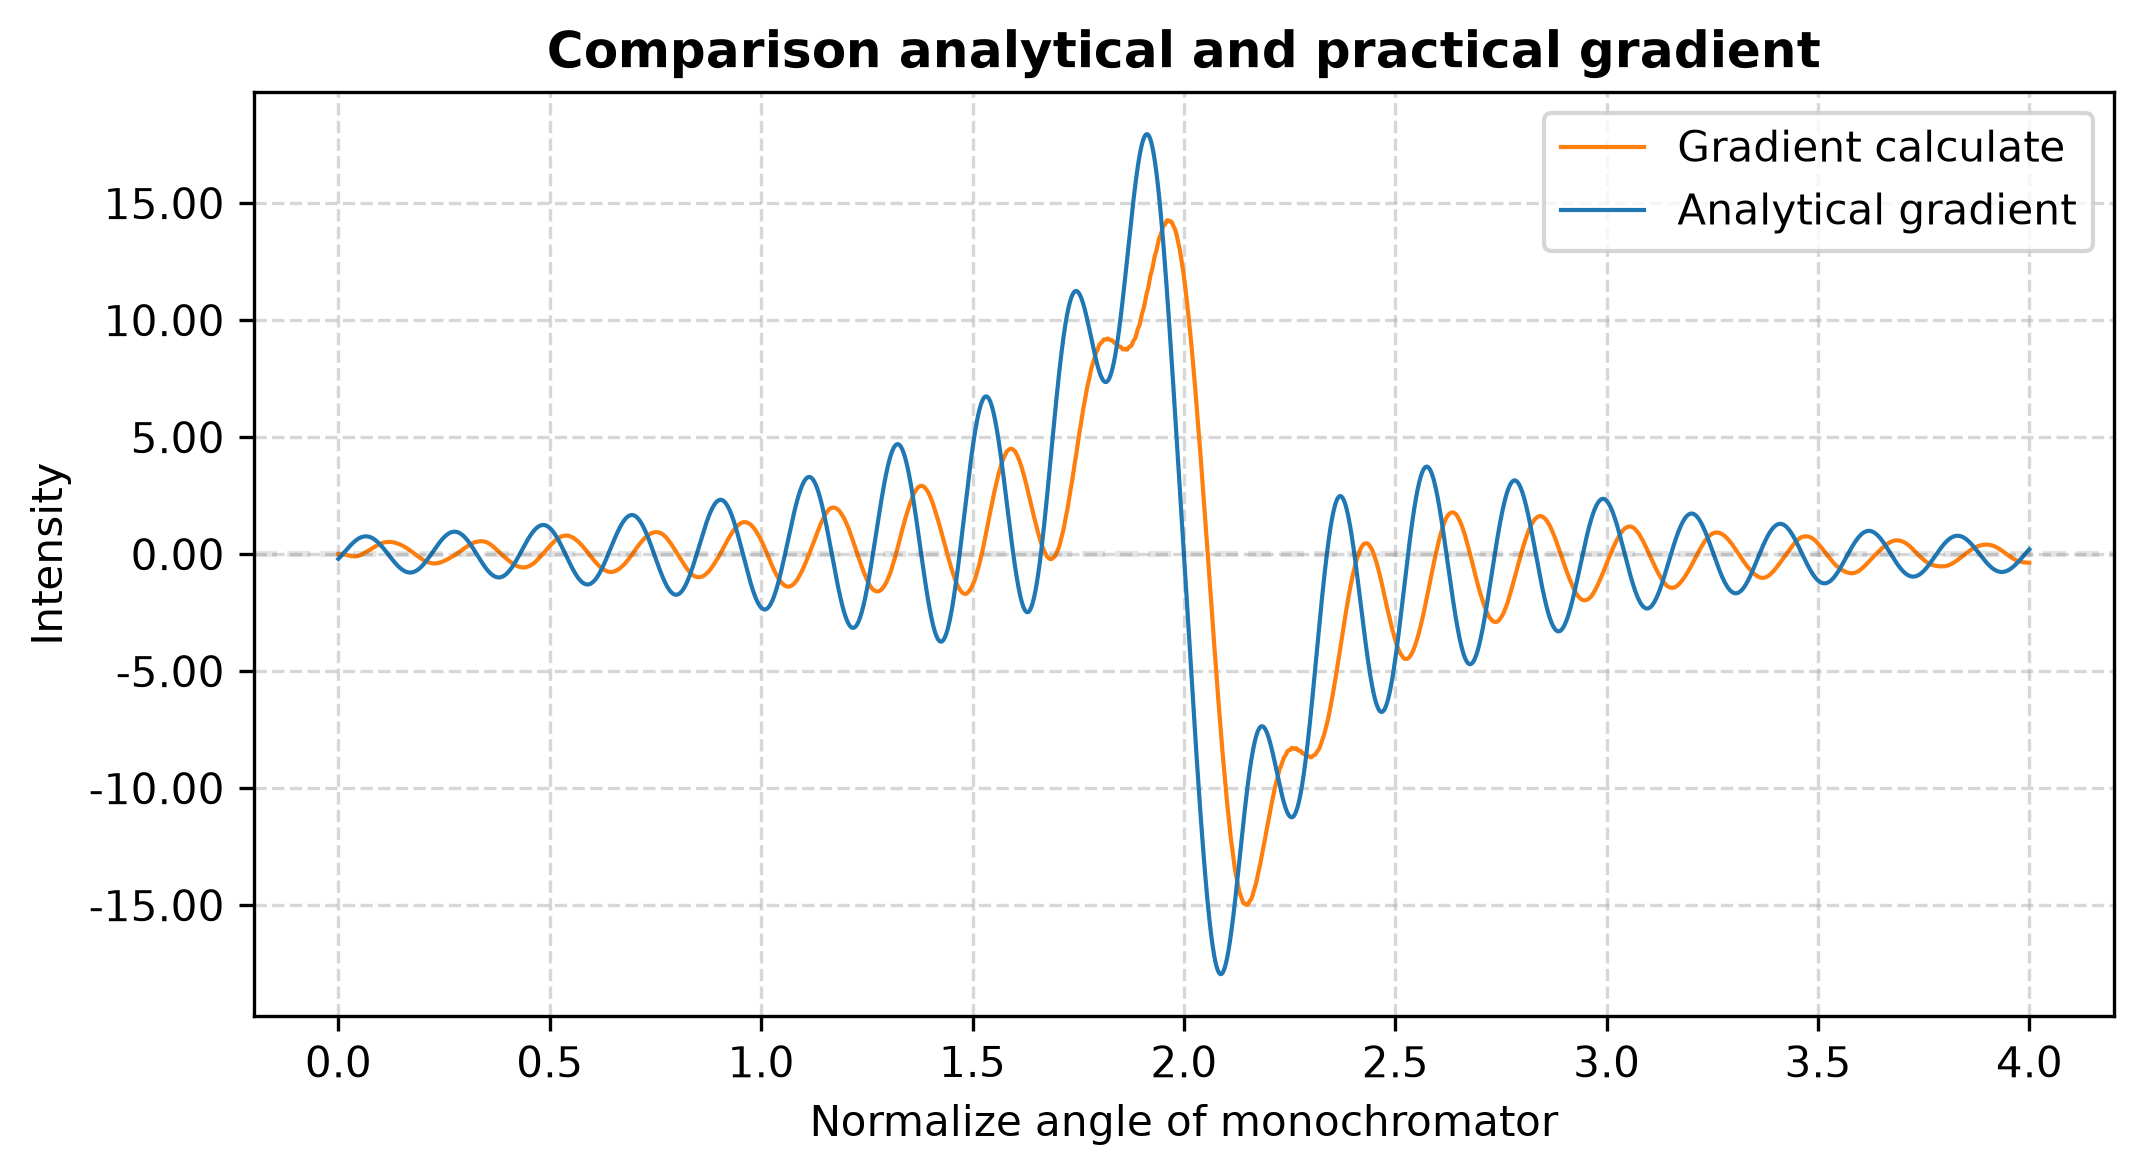
\includegraphics[width=0.85\textwidth]{img/cap 4/Comparison analytical and practical gradient.png}
    \caption{Comparison with the derivative of the simulated rocking curve function and that obtained by moving the monochromator from left to right}
    \label{fig:gradient validation}
\end{figure}

This empirically confirms the correctness of the demodulation procedure. 
Furthermore, just by looking at the graph [~\ref{fig:lockin_stages}] it is possible to distinguish:
\begin{itemize}
    \item \textbf{Zero-Crossing Precision:} The demodulated signal is represented by a classical oscillation centered on zero, which intersects the x-axis at the peak points and which corresponds to the profile of the first derivative of the oscillation curve.
    \item \textbf{Directional Polarity:} Focusing on the peak intensity position $\theta_{\text{peak}}$, if the position it'll slightly shift on the left, it is possible to see the gradient be positive with amplitude higher where the slope is stiffed. While shifting the position on the right, with the same properties, the gradient is negative. Thus the pipeline output shows the ability to recover the gradient of the intensity correctly that it will passed to the feedback controller regardless of which side of the rocking curve the system starts on.
\end{itemize}

\begin{figure}[htbp]
    \centering
    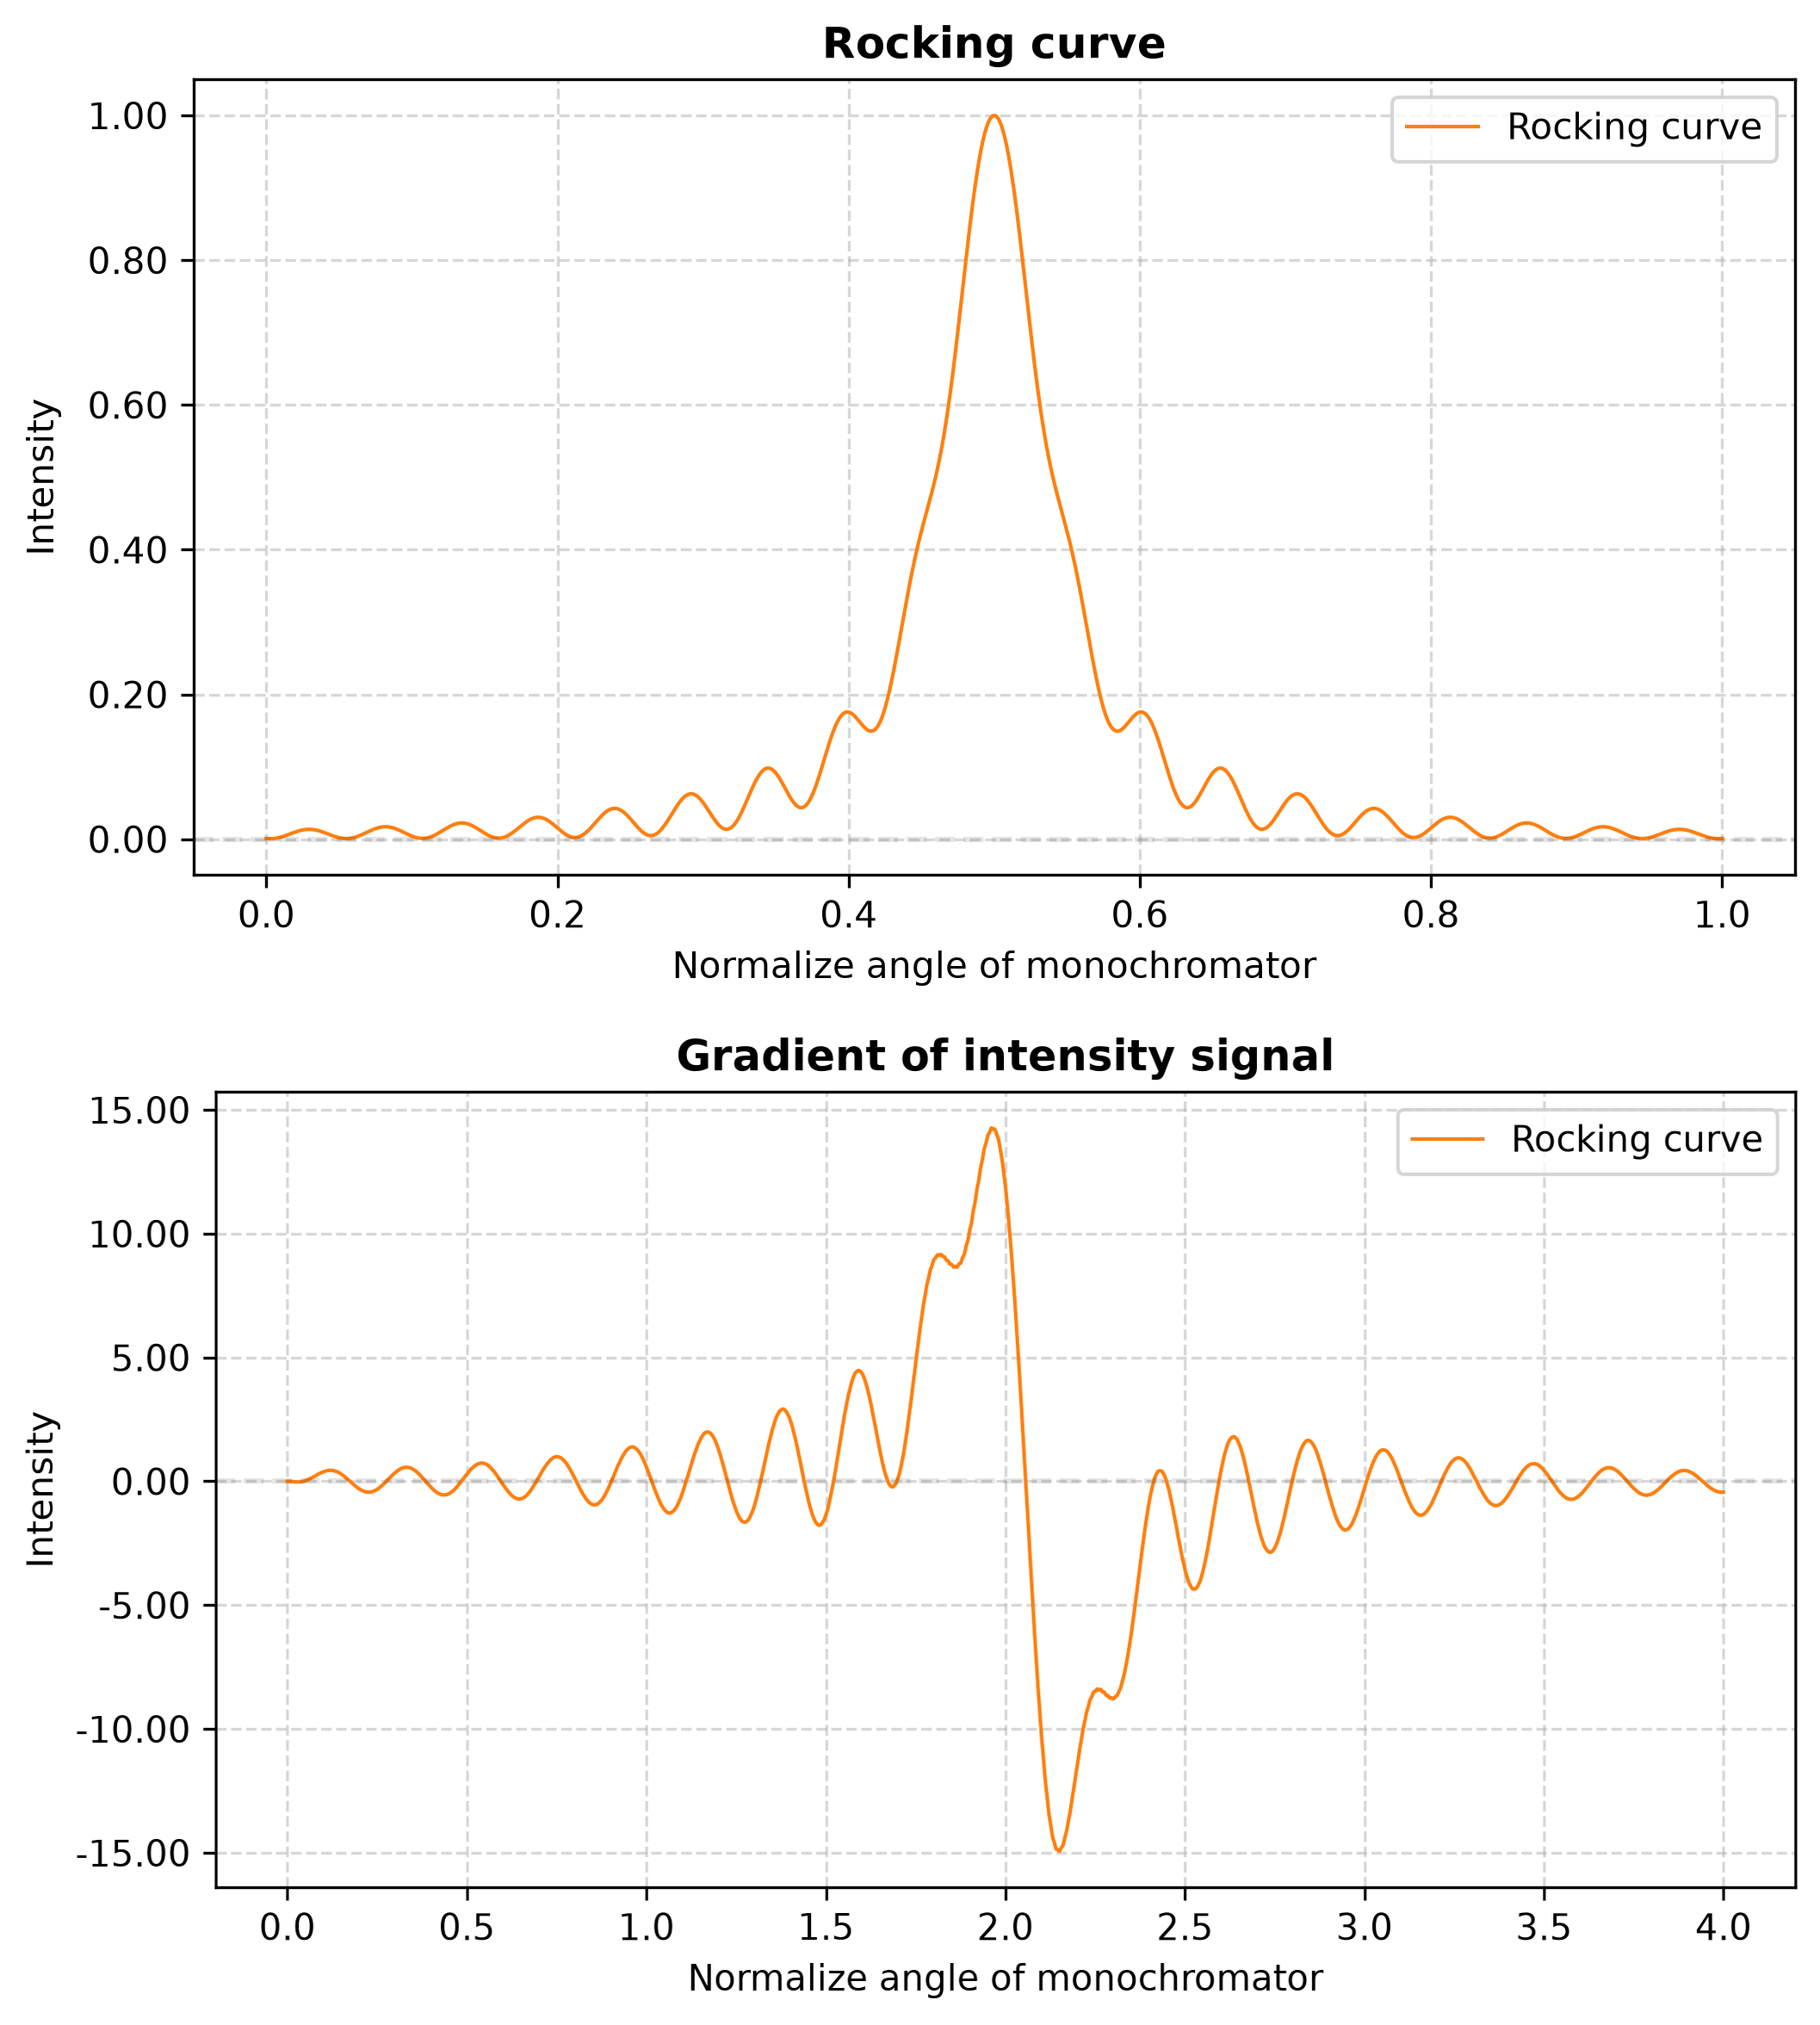
\includegraphics[width=0.85\textwidth]{img/cap 4/rocking curve and gradient calculate.png}
    \caption{Comparison between the simulated rocking curve intensity profile and the extracted lock-in gradient error signal across an angular sweep.}
    \label{fig:lockin_stages}
\end{figure}

\subsection{Steady-State Peak Holding and Dither Amplitude Trade-off}
During a simple simulation excluding all the type of low frequency drift like the thermal one, the controller was able to drive the monochromator to the right position so as to hit the peak of intensity, thus taking the first derivative to zero. 

Tests in this simple environment was useful for understanding the role of $\alpha$ and its trade-off of its magnitude:
\begin{itemize}
    \item \textbf{Small Dither Amplitudes:} 
    If where choose a small amplitude for the dither signal, The advantageous part was having a very small influence on the position by not varying the intensity too much once the peak was reached. On the other hand, however having a small amplitude cause to reduce the signal-to-noise (SNR) ratio, making the system more responsive to noise. An amplitude $\alpha$ is consider small if it is lower than $0.5$ of peak intensity.
    \item \textbf{Larger Dither Amplitudes:} 
    With larger amplitude it work the other way around, the dither signal in this case can make the control system more robust to noise at the cost of a much wider oscillation at the peak intensity once reached.
\end{itemize}
The parameter in this thesis was chosen as a compromise, so as not to have too large oscillations and at the same time not to be excessively sensitive to the noise present in the simulated environment or not.

\section{Automated Phase Calibration and Alignment}

In the previous sub section was establish the correct extraction of the intensity's gradient, but this was obtained under untrue assumptions in a real case.
In fact, in a real case, several additional factors must be taken into account, including the delay caused by the system, which in this case is the beamline.
Taking into account the delay propagation within the control system and the actual movement time of the piezo, this introduces a delay phase ($\phi_{\text{delay}}$) that will have to be managed by the control system as it could affect the gradient extraction performance and thus degrade the effectiveness of the PID.
The reason this delay affects performance is due to the way it interferes between the dither signal and the reference signal.
If the dither signal is applied at time $t$ to the piezoelectric, a certain amount of time $\Delta t$ will pass before it is detected by the BPM. Therefore, if the signal is then demodulated with the reference signal at $t$, the reference signal will be shifted by a time delay of $\Delta t$.
Since this is an instrument that will be used in a variety of settings, creating a way to automate the delay phase calculation process is necessary, using an algorithm instead of manual tuning can reduce the time of implementation of the control system while being less error prone to human error.

\subsection{The Impact of Uncompensated Phase Mismatch}

The reason why this problem was included in the thesis is related to the fact that the demodulation error is scaled with a factor of $\cos(\phi_{\text{delay}})$.
Not taking the phase delay into account can lead to different behaviors of the control system: it could decrease the amplitude of the gradient in the best case, while in the worst case, the error would change sign causing the control system to behave differently than intended.

\subsection{Automated Calibration Procedure and Quadrature Sampling}

The automatic calibration phase of the delay phase is performed early during the start-up phase of the control system, before its main control loop starts.
For simulation purposes the firmware has been modified to make the environment as realistic as possible, the changes made have been minimal and easily removable in order to return to having a firmware ready for use.
The phase delay calibration sequence follow this steps:

\begin{enumerate}
    \item \textbf{Operating Point Initialization:} First, to make the calculation more accurate, the calibration phase should position the monochromator at a point where the gradient neither changes sign nor exhibits a large difference in amplitude when the dither signal is injected. Therefore, the control system sweeps the monochromator across the entire available range, identifying the intensity peak and then positioning itself on one of the two sides.
    \item \textbf{Warm-up and Excitation Window:} Since the phase delay calculation also involves band pass and low pass filtering, the system needs to be warmed up to mitigate the disturbances generated by the initial states of the filters. After the warm-up phase, intensity samples are acquired in a predetermined time window, the sampling window.
    \item \textbf{Simultaneous In-Phase and Quadrature Mixing:} 
    During the whole sampling phase, the acquired intensity is filtered by the band pass and then multiplied by the reference sine wave and an orthogonal reference cosine wave components with frequency $\omega_d$, then both are filtered by the low pass in order to isolate their respective DC levels:
    \begin{align}
        I_{\text{in-phase}}[n] &= I_{\text{bp}}[n] \cdot \sin(\omega_d t_n) \\
        I_{\text{quadrature}}[n] &= I_{\text{bp}}[n] \cdot \cos(\omega_d t_n)
    \end{align}
    \item \textbf{Four-Quadrant Arctangent Computation:} 
    Both DCs of the components will be averaged in order to have a more accurate result, thus the system delay plus the delay injected by the filters is computed by using the four-quadrant arctangent ($\text{atan2}$) function over the mean quadrature and in-phase components:
    \begin{equation}
        \phi_{\text{delay}} = \text{atan2}\left( \frac{1}{N}\sum I_{\text{quadrature}}[n], \, \frac{1}{N}\sum I_{\text{in-phase}}[n] \right)
    \end{equation}
\end{enumerate}

\subsection{Verification of Phase Alignment Accuracy}

Tests have shown that the delay phase calibration routine is able to detect the system delay. Tests were performed with different delay times to make the test more robust.
The phase delay $\phi_{\text{delay}}$ , once calculated, will then be used by the reference signal to realign it to the dither signal.

For reference, simulations were performed with delays in the system without correcting the phase and the degradation of the control system was demonstrated.
Thanks to the calibration sequence, the reference signal is able to correctly demodulate the intensity signal having the error phase close to zero.
This also helped with system stability once the control system was up and running.

\section{Convergence Dynamics and Disturbance Rejection}

After having demonstrated the correctness of the individual phases of the pipeline and that the calculation of the delay phase was correct, it is now possible to investigate the control system as a whole and investigate the convergence to the peak intensity by testing.
Going into detail, this section also deals with the mechanical friction of the Double Crystal Monochromator (DCM) actuators and the thermal displacement.
The convergence test also includes these factors as they are the motivation that led to the beginning of this thesis.

\subsection{Closed-Loop Acquisition and Convergence Time}
In a real case scenario when the control loops is enable the starting point is already on the peak, because the main purpose of the control system is to maintain the peak intensity, but for testing the convergence in a static case where the rocking curve does not shift the start position was modified. 
It start from half from one side of the peak of intensity, so as to be equidistant from the main peak and the lateral peaks:
\begin{enumerate}
    \item \textbf{Gradient-Driven Trajectory:} The demodulated signal provide the gradient of the intensity signal and provide the direction for the controller. At each iteration, the PID attempts to adjust the position of the monochromator by applying a control signal to the piezoelectric element. The goal of the PID is to drive the piezoelectric element so as to cancel the gradient ($\text{d}I/\text{d}\theta = 0$).
    \item \textbf{Settling Behavior and Overshoot:} Tuning the parameter of the PID ($K_p,K_i,K_d$) was made manual with a try-and-error approach, they where choose in a way to have a controller to converge fast and guarantee stability once the peak is reached.
    As mention before in simulation telemetry, the control system reach convergence at time of [~\ref{fig:feedback control loop response}] it stabilizes cautiously with a slight initial overshoot without endlessly oscillation or trying to achieve its goal even once reached.
\end{enumerate}

\begin{figure}[htbp]
    \centering
    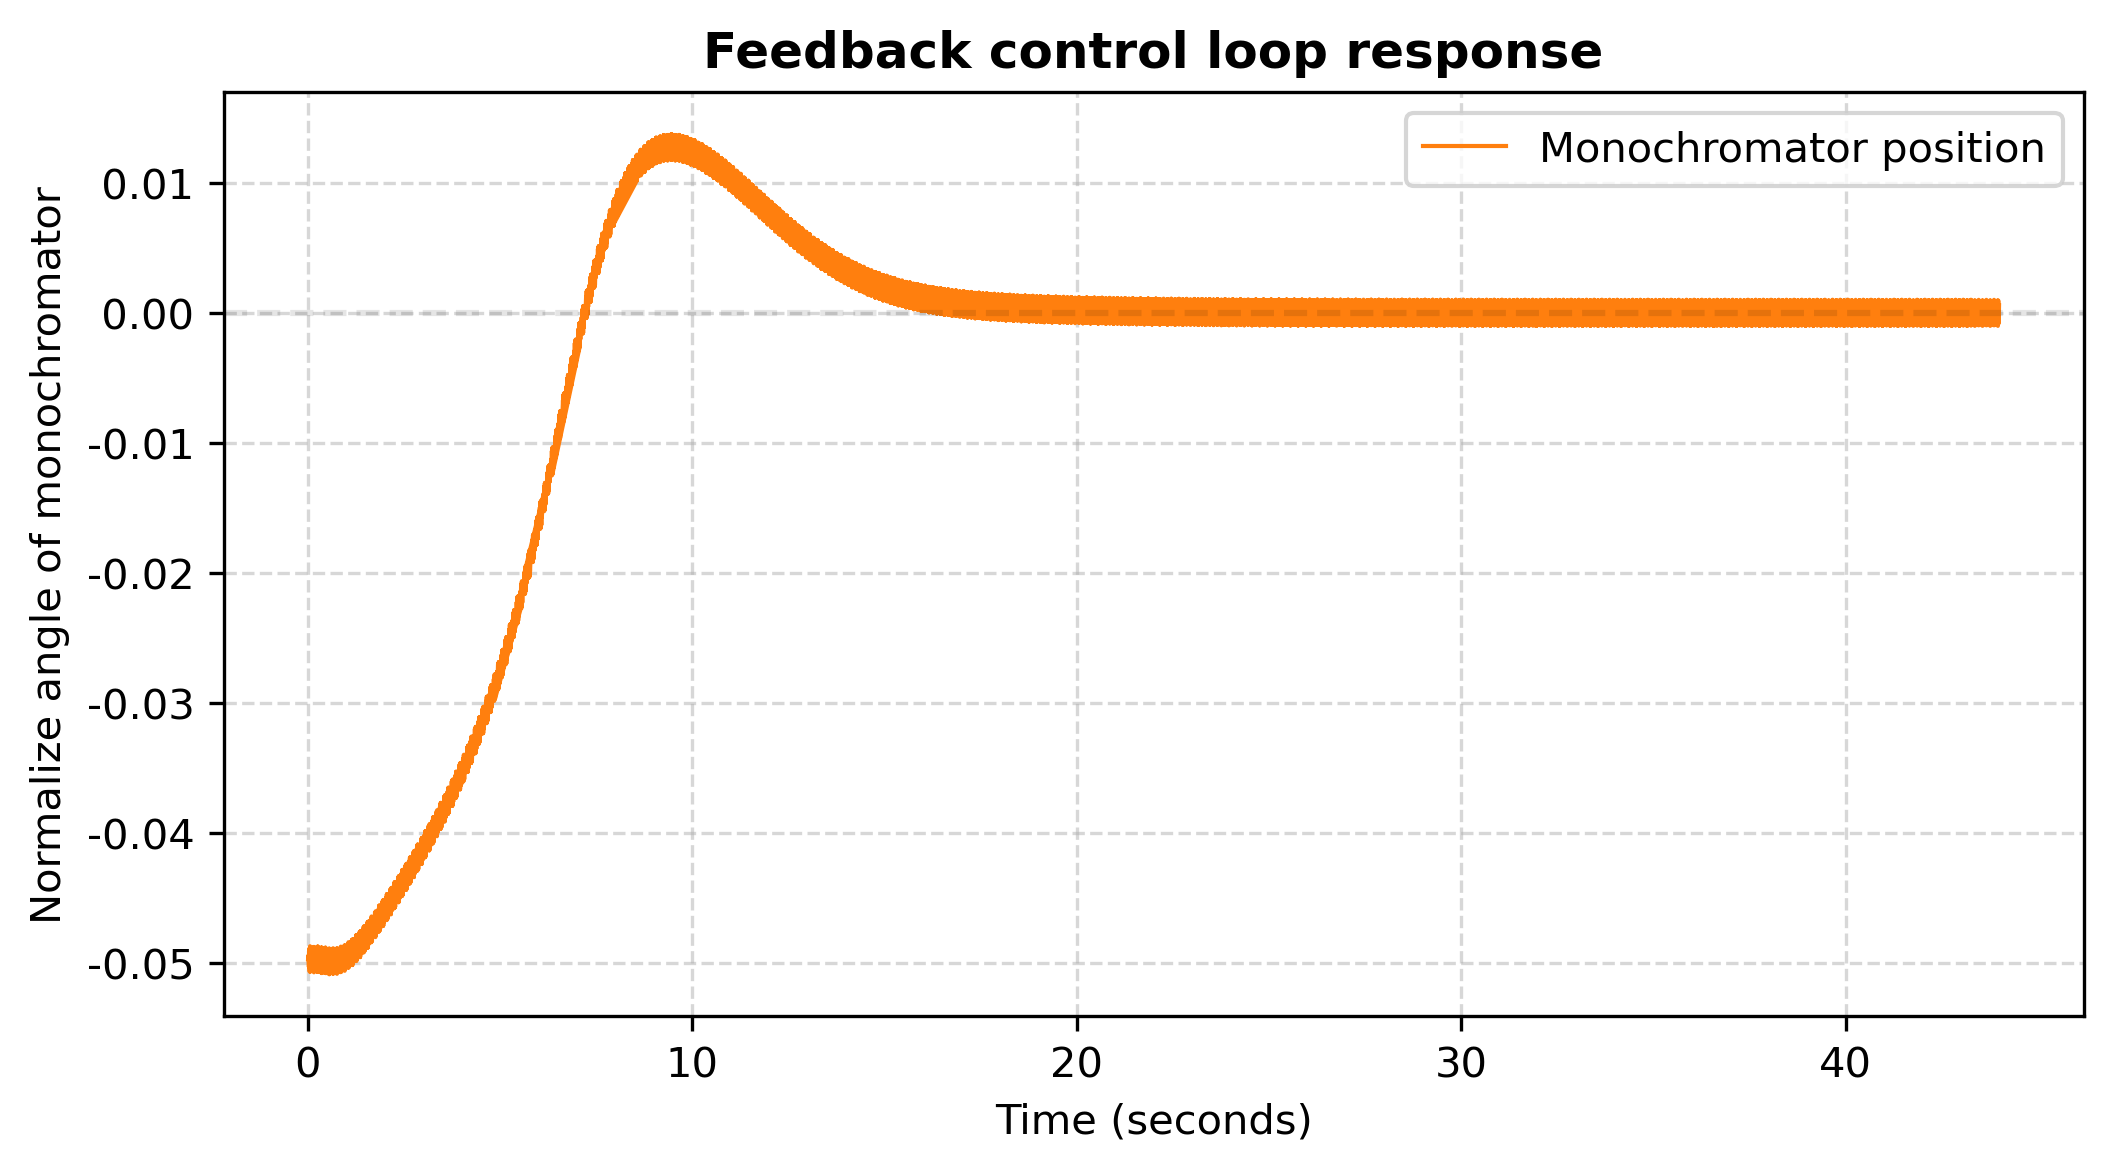
\includegraphics[width=0.85\textwidth]{img/cap 4/Feedback control loop response.png}
    \caption{Controller response to reach set point when monochromator is at position -0.045.}
    \label{fig:feedback control loop response}
\end{figure}

\subsection{Thermal and Mechanical Disturbance Rejection}

Optical component inside a real synchrotron beamline, during long experiments the crystal lattice can expand or contract if change its temperature. 
This leads to a shift in the rocking curve and consequently to a shift in the intensity peak.
To emulate the thermal displacement component, it must be translated into a time-varying displacement. 
Knowing that thermal drift is a low-frequency phenomenon, the equation describing the thermal displacement for the simulation is a sine wave with frequency of $0.001\text{kHz}$, so the peak of the rocking curve shifts by the sine wave.

\begin{itemize}
    \item \textbf{Tracking Drift Dynamics:} 
    If not taken into account, thermal drift causes a loss of beam intensity as the peak moves away from the position of the monochromator which instead remains stationary.
    \item \textbf{Closed-Loop Compensation:} 
    Instead, if the control system is activated, it is able, as has already been demonstrated, to detect the variation in the derivative of the intensity.
    The PID controller, receiving the derivative of the intensity, calculates the amount of movement needed by the piezoelectric to continue following the migrating peak and must do so for extended periods of operation, maintaining stability at the peak intensity.
\end{itemize}

\begin{figure}[htbp]
    \centering
    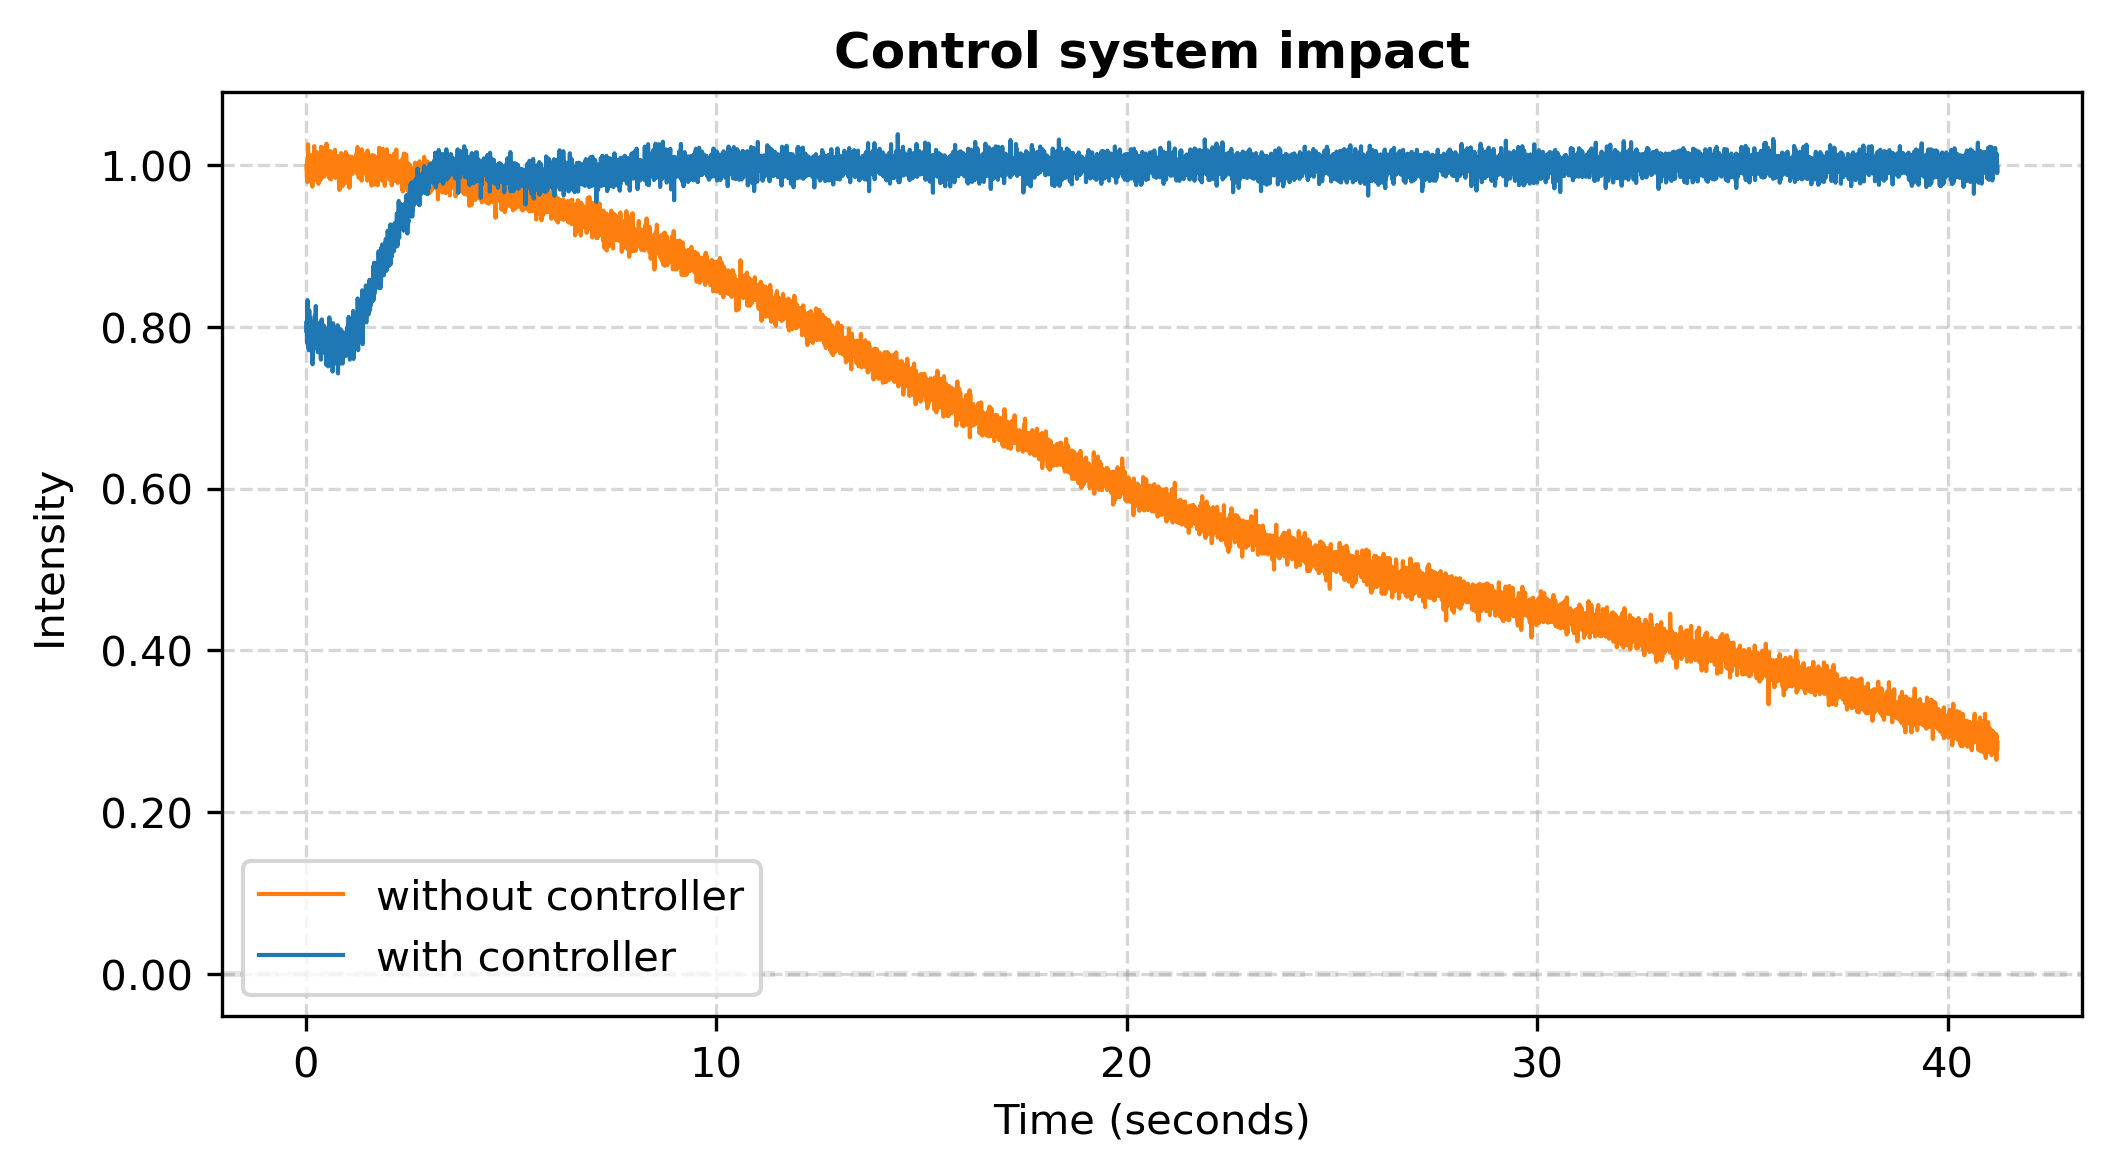
\includegraphics[width=0.85\textwidth]{img/cap 4/Control system impact.png}
    \caption{The impact of the control system in case of noise and thermal drift against keeping the monochromator position fixed.}
    \label{fig:disturbance_rejection}
\end{figure}

\subsection{Steady-State Stability and Jitter Analysis}

Once peak intensity was reached, the control system demonstrated robust steady-state stability.
Even if the controller reach his set point, control signal still will not be zero due to the dither amplitude ($\alpha$) and the low-pass filter bandwidth.

Since the main circuitry of the control system is executed within the FPGA using an interrupt service routine (ISR), the control is called at deterministic intervals, thus eliminating jitter.
The interrupt service routine is triggered by a signal emitted at a frequency of $100\text{ kHz}$.

\section{Driver Telemetry and Supervisory GUI Verification}

To be able to view the internal behavior of the control system through parameters such as the intensity derivative, the control signal, or the intensity itself, it was necessary to extract the telemetry data and implement an interface to display them.
Based on the existing implementation of communication between the FPGA and the host PC, which operates via a shared map memory, it was possible to use some unreserved slots for extracting telemetry data.
Although a graphical implementation for displaying telemetry data was already available, it was necessary to build another framework to analyze this data more practically, as Python is easier for data analysis than the Qt framework for C/C++.

\subsection{Python-Based Telemetry and Pipeline Analysis Framework}

Another rejected solution was to debug within the Quartus II development environment, but this presented significant debugging constraints, so a parallel testing pipeline was constructed in Python:
\begin{itemize}
    \item \textbf{Data Logging and Export:} 
    By making the data available in memory, it was sufficient to find the indexes whose slots were reserved for the simulation data. The calls to read the data were performed using an already developed library.
    \item \textbf{Online Validation:}  The data analysis was performed after a visual validation of the control system behavior inside a control panel, which helped in the implementation phase of the FPGA and the tuning of the parameters present within the control system. Figure[~\ref{fig:monitoring panel}]

\begin{landscape}
\begin{figure}[p]
    \centering
    \includegraphics[
        width=\linewidth,
        height=0.85\textheight,
        keepaspectratio
    ]{img/cap 4/Monitoring panel.png}
    \caption{Control panel for monitoring the control system under development, with access to specific memory slots.}
    \label{fig:monitoring panel}
\end{figure}
\end{landscape}
    
    \item \textbf{Offline Validation and Plotting:} 
    Before implementing the solution on the FPGA, it was simulated and tested in a more practical environment to make the implementation cleaner once the results were obtained.
    Python was useful because the easy modifications to the code led to faster development and the ability to create graphs using scientific packages (such as NumPy, SciPy, and Matplotlib).
    It was also useful for calculating the coefficients of the bandpass and lowpass filters.
    Furthermore, the framework for real-time visualization of the simulation on the FPGA made it possible to acquire the data for the analyses mentioned in the previous sections.
\end{itemize}

\subsection{Supervisory GUI Integration and Real-Time Visibility}
For a real-world implementation of the system at a physical facility, the framework created in Python cannot be used, as its purpose is only to simulate the physical system.
The local GUI already developed in Qt C++ performs various functions for monitoring and tuning the control system previously developed for position control:
\begin{itemize}
    \item \textbf{Real-Time Gradient and Rocking Curve Rendering:} 
    The GUI already provides the ability to view various system parameters such as the position of the beam and its intensity, now in addition, it is possible to observe the trend of the first derivative, giving operators immediate visual confirmation of whether the system is locked onto the peak.
    \item \textbf{Dynamic Parameter Configuration:} 
    Through a communication channel other than shared memory, the mailbox allows information to be shared between the host PC and the FPGA. This communication channel was designed to avoid the need to continuously send data, as happens with shared memory, for example.
    In the mailbox, it is used to set the parameters of the PID used for position control.
\end{itemize}

\begin{landscape}
\begin{figure}[p]
    \centering
    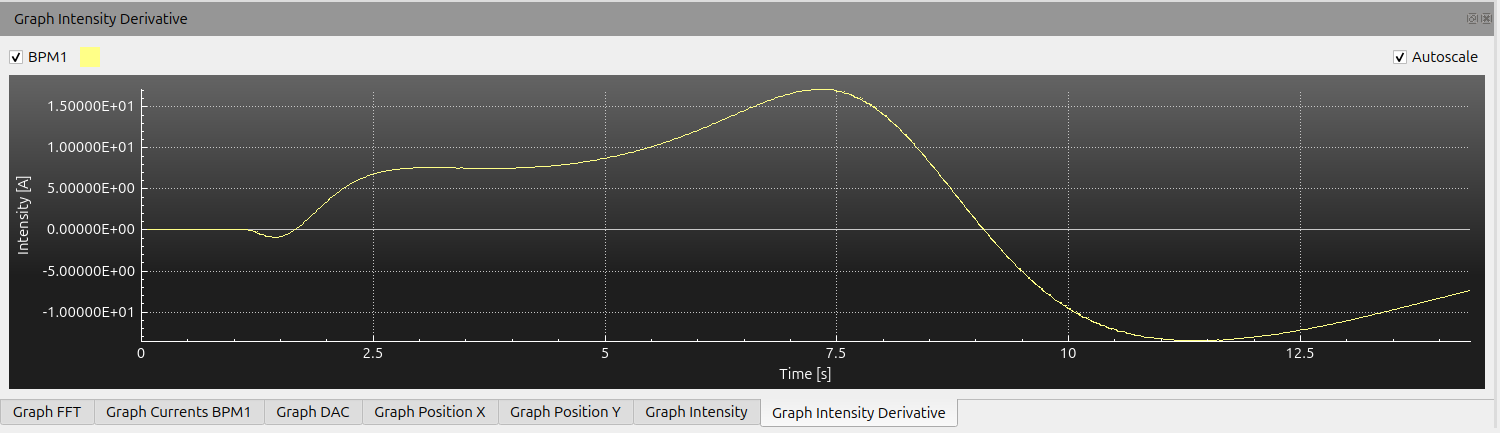
\includegraphics[
        width=\linewidth,
        height=0.85\textheight,
        keepaspectratio
    ]{img/cap 4/local GUI.png}
    \caption{Prototype of the integrated monitoring interface within the local Qt/C++ GUI.}
    \label{fig:disturbance rejection}
\end{figure}
\end{landscape}

Through a communication channel other than shared memory, the mailbox allows information to be shared between the host PC and the FPGA. This communication channel was designed to avoid the need to continuously send data, as happens with shared memory, for example.
In the mailbox, it is used to set the parameters of the PID used for position control.

\section{Summary of Validation Results}

The proposed system was tested to validate it and demonstrate its capability in maintaining the monochromator position that corresponds to the maximum beam intensity.
Testing the system in a real case scenario proved impractical, as the synchrotrons using the equipment are few and not always available.
So instead of having a real plant for the tests, it was simulated by mocking the FPGA input intensity.
In this way it was possible to test the system under different circumstances by adding noise, phase delay and thermal drift.

Before going to test the system behavior, it was necessary to analyze the FPGA implementation to ensure that it respected the execution time and memory constraints.

Afterwards, the individual stages of the pipeline were analyzed to verify that each of them performed its task correctly.
The results showed the correct filtering of the bandpass filter by isolating the dither signal, and the demodulation led to a correct extraction of the intensity gradient.

Even if all the stages taken alone were proven correct, in real case scenario the pipeline might not work because it doesn't take the system's delay time into account. 
if it is not taken into consideration, there's a risk that demodulation will be incorrect.
Tests have demonstrated the correct calculation of the phase delay.

The control system correctly identified the direction to take to adjust the monochromator's position to follow the intensity peak. 
Furthermore, the PID was tuned to achieve the desired behavior and it was demonstrated its stability once the maximum was reached, even when thermal drift was present. 
Tests on the control system concluded by comparing it with a system operating without feedback, showing showing the advantage of having an active peak tracking system.

The tests were accompanied by a control panel built specifically for the tests, which allowed monitoring the intermediate stages of the control system. Meanwhile, the intensity gradient display was integrated into the local GUI.

The results demonstrated the validity of the proposed solution implemented inside the FPGA.
However, this control system should be tested with a real plant, in order to verify its behaviour under real operating conditions.

\newpage